\documentclass[serif, aspectratio=169]{beamer}
%\documentclass[serif]{beamer}  % for 4:3 ratio

\usepackage[T1]{fontenc} 
\usepackage[utf8]{inputenc}
\usepackage{fourier} % see "http://faq.ktug.org/wiki/uploads/MathFonts.pdf" for other options
\usepackage{hyperref}
\usepackage{latexsym,amsmath,xcolor,multicol,booktabs,calligra}
\usepackage{graphicx,pstricks,listings,stackengine}
\usepackage{lipsum}
\usepackage{../HKUSTstyle}

%imports customs%
\usepackage{caption}    % for subfigures
\usepackage{subcaption} % for subfigures
\usepackage{ragged2e}
\usepackage{booktabs,makecell}
\usepackage{colortbl}
\usepackage{multirow}
\usepackage{cite}
\usepackage{tcolorbox}
\usepackage[sort,authoryear]{natbib}

\author{Julien Bezançon}

\title{Découverte du Traitement Automatique des Langues}
\subtitle{Hors-série 1~: Les expressions régulières}

\institute{julien.bezancon@univ-lorraine.fr / \url{https://julienbez.github.io}}

\date{}

% defs
\def\cmd#1{\texttt{\color{red}\footnotesize $\backslash$#1}}
\def\env#1{\texttt{\color{blue}\footnotesize #1}}

% set colors
\definecolor{hkustyellow}{RGB}{167, 131, 55}
\definecolor{hkustblue}{RGB}{0, 56, 116}
\definecolor{hkustred}{RGB}{209, 51, 59}

\lstset{
    basicstyle=\ttfamily\small,
    keywordstyle=\bfseries\color{deepblue},
    emphstyle=\ttfamily\color{deepred},    % Custom highlighting style
    stringstyle=\color{deepgreen},
    numbers=left,
    numberstyle=\small\color{halfgray},
    rulesepcolor=\color{red!20!green!20!blue!20},
    frame=shadowbox,
}

\begin{document} %  --- --- --- --- --- --- --- --- --- --- --- --- 

\begin{frame}[noframenumbering,plain]
    \titlepage
    \vspace*{-0.6cm}
    \begin{figure}[htpb]
        \begin{center}
            \hspace{0.3cm}
            
\includegraphics[width=0.7\columnwidth]{../../../IMAGES/loria_idmc.png}
        \end{center}
    \end{figure}
\end{frame}

% \begin{frame}    
%     \tableofcontents[sectionstyle=show,
%     subsectionstyle=show/shaded/hide,
%     subsubsectionstyle=show/shaded/hide]
% \end{frame}

\section{Avant de commencer...}

\begin{exoframe}{}
    \begin{center}
        \Large
        De quoi avons-nous discuté lors du derniers cours ? \\
        Avez-vous des questions ?
    \end{center}
\end{exoframe}

\begin{frame}{Chronologie du TAL}
    \begin{figure}
        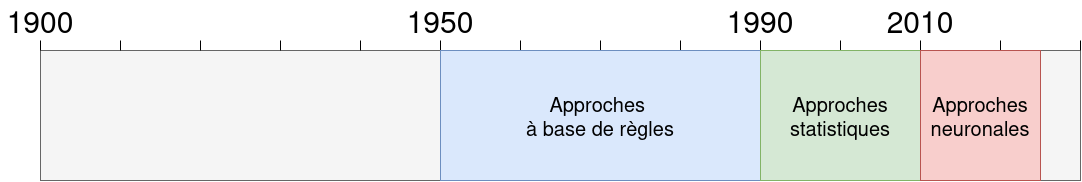
\includegraphics[width=1\columnwidth]{../../../FIGURES/découverte_tal/tal_chronologie.png}
    \end{figure}
\end{frame}

\section{Approches à base de règles}

\begin{frame}{Approches à base de règles}
    \begin{block}{Objectifs}
        \begin{itemize}
            \item On veut traiter du langage avec des machines
            \item On choisi de donner des règles à ces machines
        \end{itemize}
    \end{block}
    \begin{block}{C'est quoi une règle ?}
        \begin{itemize}
            \item Une analyse faite sur un phénomène régulier
            \item Langue = groupe de règles implicites
        \end{itemize}
    \end{block}
    \vfill
    \begin{center}
        \Large
        Une règle doit être exprimée en langage logique \\
        pour être interprétée par une machine.
    \end{center}
\end{frame}

\begin{exoframe}{}
    \begin{center}
        \Large
        Quelles sont les règles pour définir un mot du français ? \\
        \pause
        Pouvez-vous les formaliser en langage logique ?
    \end{center}
\end{exoframe}

\begin{frame}{Définir un mot}
    \begin{block}{Règles du mot}
        \begin{itemize}
            \item Suite de caractères
            \item Délimité par des espaces
            \item Possède un sens / un signifié
        \end{itemize}
    \end{block}
    \vfill
    \begin{block}{Cas problématiques}
        \begin{itemize}
            \item Tire-bouchon $\Rightarrow$ un seul mot ?
            \item Pomme de terre $\Rightarrow$ un seul mot ?
            \item IDMC $\Rightarrow$ suite de caractères, donc c'est un mot ?
        \end{itemize}
    \end{block}
\end{frame}

\begin{frame}{Rappel~: la tokénisation}
    \begin{block}{Objectif(s)}
        \begin{itemize}
            \item Découper un énoncé en tokens
            \item Idéalement, 1 mot = 1 token
            \item Permet de traiter chaque mot indépendamment
        \end{itemize}
    \end{block}
    \begin{block}{Exemples}
        \begin{itemize}
            \item \wordbox{Les} \wordbox{étudiants} \wordbox{mangent} \wordbox{un} \wordbox{kebab}
            \item \wordbox{pomme de terre} ou \wordbox{pomme} \wordbox{de} \wordbox{terre} ?
            \item \wordbox{tire-bouchon} ou \wordbox{tire} \wordbox{-} \wordbox{bouchon} ?
            \item \wordbox{pierre} \wordbox{qui} \wordbox{roule} \wordbox{n'}\wordbox{amasse} \wordbox{pas} \wordbox{mousse} ?
        \end{itemize}
    \end{block}
\end{frame}

%faire slide ou on explique pourquoi c'est cool
%slide interprétabilité + extension (ou intension)
%on a pas besoin de beaucoup de données pour créer des règles
%on peut même générer du langage à partir de règles, même si les résultats seront limités à des énoncés réguliers et simples
%les règles sont plus ou moins généralisables
%si une règle ne s'applique pas dans un cas particulier, on peut l'ajuster avec une nouvelle règle
%inconvénient : nécéssite beaucoup de connaissances et de temps, ya beaucoup de cas particuliers

\begin{frame}{En somme...}
    \begin{block}{}
        \begin{itemize}
            \item 
        \end{itemize}
    \end{block}
\end{frame}

\end{document}

    % \begin{table}
    %     \centering
    %     \renewcommand{\arraystretch}{1.5}  
    %     \begin{tabular}{|c|c|c|c|}
    %         \hline
    %         Interprétabilité & Couverture & Données & Ressources \\
    %         \hline
    %         ++ & + & -\nothing{}- & - \\
    %         \hline
    %     \end{tabular}
    % \end{table}